%-----Main FIle------
%For Detail check out - http://firesofmay.blogspot.com/2011/10/latex-project-report-template
%CHANGE THESE Settings ONLY IF YOU KNOW WHAT YOU DOING

\documentclass[12pt,a4paper]{report}

%adjust your page margins here
\usepackage[top=0.70in, bottom=0.70in, left=0.8in,right=0.80in]{geometry} % setting the page alignment with this package
\usepackage[pdftex]{graphicx} %for embedding images
%\usepackage[hyphens]{url} %for proper url entries
\usepackage[dvips, bookmarks,  colorlinks=false]{hyperref} %for creating links in the pdf version and other additional pdf attributes, no effect on the printed document
\hypersetup{%
    pdfborder = {0 0 0}
}
\usepackage[final]{pdfpages} %for embedding another pdf, remove if not required
\usepackage{float} %used for figure placement with H as a parameter
%\usepackage[hyphens]{url}
%\usepackage{hyperref}
\usepackage{pslatex} % for times new roman, old package, but works
\usepackage{array} % for making text bold in table
\usepackage{setspace}
\usepackage{float}
\usepackage{enumerate}
%\usepackage{indentfirst}

\usepackage[font=small,labelfont=bf]{caption}
\def\figurename{\textbf{Figure }}
%\renewcommand{\thefigure}\textbf{{\arabic{section}.\arabic{figure}}}
%\def\thefigure{\@arabic\c@figure}
%\def\fnum@figure{\figurename\ \textbf{\thefigure}}
%\setlength{\parindent}{1cm}

%For inserting Python Code
\usepackage{listings}
\usepackage{color}

%\usepackage[a4,frame,center]{crop}

\definecolor{dkgreen}{rgb}{0,0.6,0}
\definecolor{gray}{rgb}{0.5,0.5,0.5}
\definecolor{mauve}{rgb}{0.58,0,0.82}
 
\lstset{ %
  language=Python,                % the language of the code
  basicstyle=\footnotesize,           % the size of the fonts that are used for the code
  numbers=left,                   % where to put the line-numbers
  numberstyle=\tiny\color{gray},  % the style that is used for the line-numbers
  stepnumber=1,                   % each line is numbered
  numbersep=5pt,                  % how far the line-numbers are from the code
  backgroundcolor=\color{white},      % choose the background color. You must add \usepackage{color}
  showspaces=false,               % show spaces adding particular underscores
  showstringspaces=false,         % underline spaces within strings
  showtabs=false,                 % show tabs within strings adding particular underscores
  frame=single,                   % adds a frame around the code
  rulecolor=\color{black},        % if not set, the frame-color may be changed on line-breaks within not-black text (e.g. commens (green here))
  tabsize=2,                      % sets default tabsize to 2 spaces
  captionpos=b,                   % sets the caption-position to bottom
  breaklines=true,                % sets automatic line breaking
  breakatwhitespace=false,        % sets if automatic breaks should only happen at whitespace
  title=\lstname,                   % show the filename of files included with \lstinputlisting;
                                  % also try caption instead of title
  keywordstyle=\color{blue},          % keyword style
  commentstyle=\color{dkgreen},       % comment style
  stringstyle=\color{mauve},         % string literal style
  escapeinside={\%*}{*)},            % if you want to add a comment within your code
  morekeywords={*,...}               % if you want to add more keywords to the set
}

%%%%For inserting Python Code Over



%For the header and footer
\usepackage{fancyhdr}
\fancypagestyle{plain}{%
%\fancyhf{} % clear all header and footer fields
\fancyfoot[L]{\emph{Department of Computer Engineering, JSCOE, Pune}} % except the center
\fancyfoot[R]{\thepage}
\renewcommand{\headrulewidth}{0.4pt}
\renewcommand{\footrulewidth}{0.4pt}
%\setlength{\headsep}{0pt}
%\addtolength{\voffset}{-5pt}
%\setlength{\topmargin}{20pt}
%\setlength{\textheight}{592pt}
}

\pagestyle{fancy}
%\lhead{Chapter \thechapter}
%\renewcommand{\chaptermark}[1]{% 
\rhead{\emph{Android Synchronization Manager}}
%\markboth{#1}{}} 

\fancyfoot[LO,LE]{\emph{Department of Computer Engineering, JSCOE, Pune}}
\cfoot{}
\fancyfoot[RO, RE]{\thepage}
\renewcommand{\headrulewidth}{0.4pt}
\renewcommand{\footrulewidth}{0.4pt}
%For the header and footer Over

% Altering the Index Page Title
%\renewcommand{\contentsname}{\begin{center}\textsc{University Of Pune \\2011 - 2012}\\[1cm]Index\end{center}} 


%GLOBAL SETTINGS OVER, DOCUMENT BEGINS
\begin{document}
%\begin{spacing}{0}{
%Renames "Bibliography" to "References" on ref page
\renewcommand\bibname{References}
\lhead{ }

%\renewcommand{\thefigure}{\arabic{\textbf{section}}.\arabic{\textbf{figure}}}}

%FROM HERE YOUR PAGES START GETTING ADDED

% includes the cover page
%2nd page after the title page

\newpage


\begin{center}
\thispagestyle{empty}


\Large{\textbf{A\\Project Report On}}\\[0.7cm]
\Large{\textsc {\textbf{Android Synchronization Manager}}}\\[0.5cm]
%Example
%\Huge{\textsc {\textbf{A case study on linux}}}\\[1.0cm] % NOTE YOU HAVE TO REMOVE THE << >> ALSO!! That's just a placeholder here.
\Large{\textbf{Submitted By}}\\[0.5cm]
\begin{table}[h]
\centering
\begin{tabular}{>{\bfseries}lc>{\bfseries}r}
Parikshit Ghodake & & B8404217\\ %Example B-1231414
Imran Ahmed & & B8404221\\ %Example B-1231414
Akshay Khole & & B8404237\\ %Example B-1231414
Muneeb Shaikh & & B8404259\\ %Example B-1231414
\end{tabular}
\end{table}
\large{Under the guidance of}\\[0.5cm]
\Large{\textbf{Prof. H. A. Hingoliwala}}\\[0.4cm]
\large{\emph{In partial fulfilment of}}\\
\LARGE{\textbf{Bachelor of Engineering}}
\LARGE{{{(}Computer Engineering{)}}\\[0.5cm]
\LARGE{{[}May 2012{]}}\\
\Large{\emph{AT}}\\[0.2cm]


% Bottom of the page

%MODIFY THE LOGO/DEPARTMENT NAME/COLLEGE NAME/ADDRESS IF YOU HAVE TO, ELSE LEAVE IT

\includegraphics[scale=0.5]{project/jscoe_logo}\\
\large{\textbf{Department of Computer Engineering}}\\
\LARGE{\textbf{Jayawantrao sawant college of engineering}}\\
\Large{\textbf{Hadapsar, Pune – 411028}}\\[0.5cm]
\Large{\textbf{Affiliated to}}\\[0.5cm]

\includegraphics[scale=5.0]{project/uop-logo}\\
\LARGE{\textbf{University of Pune}}
\newpage

\end{center}

% Bottom of the page
%\begin{flushright}
%Faculty In-charge\\[1.5cm]
%Course Co-ordinator\\[1.0cm]
%\end{flushright}

%\begin{flushleft}
%Date:
%\end{flushleft}

\newpage

%2nd page after the title page

\newpage


\begin{center}
\thispagestyle{empty}


\Large{\textbf{A PROJECT REPORT\\ON}}\\[0.7cm]
\Large{\textsc {\textbf{``ANDROID SYNCHRONIZATION MANAGER''}}}\\[0.5cm]
%Example
%\Huge{\textsc {\textbf{A case study on linux}}}\\[1.0cm] % NOTE YOU HAVE TO REMOVE THE << >> ALSO!! That's just a placeholder here.
\Large{\textbf{\\Submitted to}}
\LARGE{\textbf{\\UNIVERSITY OF PUNE\\}}
\large{\textbf{\\In Partial Fulfilment of the Requirement for the Award of\\}}
\LARGE{\textbf{\\BACHELOR'S DEGREE IN\\COMPUTER ENGINEERING}}
%\LARGE{\textbf{\\COMPUTER ENGINEERING \\}}
\vspace{0.5cm}
\Large{\textbf{\\BY}}\\[0.5cm]
\begin{table}[h]
\centering
\Large{
\begin{tabular}{>{\bfseries}lc>{\bfseries}r}
Parikshit Ghodake & & B8404217\\Imran Ahmed & & B8404221\\Akshay Khole & & B8404237\\Muneeb Shaikh & & B8404259\\
\end{tabular}}
\end{table}
%\large{UNDER THE GUIDANCE OF}\\[0.5cm]
%\Large{\textbf{PROF. }}\\[0.4cm]
%\LARGE{{[}May 2012{]}}\\
%\Large{\emph{AT}}\\[0.2cm]


% Bottom of the page

%MODIFY THE LOGO/DEPARTMENT NAME/COLLEGE NAME/ADDRESS IF YOU HAVE TO, ELSE LEAVE IT

\includegraphics[scale=0.5]{project/images/jscoe_logo}\\
\large{\textbf{DEPARTMENT OF COMPUTER ENGINEERING}}\\
\Large{\textbf{JAYAWANTRAO SAWANT COLLEGE OF ENGINEERING}}\\
\large{\textbf{HADAPSAR, PUNE - 28}}
\large{\textbf{\\2011-2012}}\\[0.5cm]
\Large{\textbf{AFFILIATED TO}}\\[0.5cm]

\includegraphics[scale=5.0]{project/images/uop-logo}\\
\LARGE{\textbf{UNIVERSITY OF PUNE}}
\newpage

\end{center}

% Bottom of the page
%\begin{flushright}
%Faculty In-charge\\[1.5cm]
%Course Co-ordinator\\[1.0cm]
%\end{flushright}

%\begin{flushleft}
%Date:
%\end{flushleft}

\newpage

% includes the certificate page
%\chapter*{}
%\lipsum
\begin{center}
\thispagestyle{empty}

\LARGE{\textbf{Jayawantrao Sawant College of Engineering}} \\ 
\large{\textbf{Department of Computer Engineering}}\\
\large{\textbf{Hadapsar, Pune – 411028}}\\[0.5cm]


\includegraphics[scale=0.5]{project/images/jscoe_logo}\\[0.5cm]

{\Huge \textbf{CERTIFICATE}}\\[0.5cm]
\end{center}
\linespread{1.13}
%\begin{center}
\large{\centering{This is certify that the dissertation entitled}\\[0.2cm]
%\end{center}
\textbf{\Large{\centering{``ANDROID SYNCHRONIZATION MANAGER''}}}\\[0.2cm]
\centering{submitted by}\\[0.2cm]
\begin{table}[h]
\centering
\large{
\begin{tabular}{>{\bfseries}lc>{\bfseries}r}
Parikshit Ghodake & & B8404217\\Imran Ahmed & & B8404221\\Akshay Khole & & B8404237\\Muneeb Shaikh & & B8404259\\
\end{tabular}}
\end{table}
%\textbf{
 is a record of bonafide work carried out by them, in the partial
 fulfilment of the requirement for the award of Degree of Bachelor of
 Engineering (Computer Engineering) at Jayawantrao Sawant College of
 Engineering, Pune under the University of Pune. This work is done
 during year 2011-2012, under our guidance.}\\[0.5cm]
\large{\textbf{Date:\hspace*{1.0cm}/\hspace*{1.0cm}/}}\\
\begin{spacing}{0}
%\large{---------------------------------}\\
\vspace{3.0cm}
%\large{--------------------------------}\hspace*{1.5in}
\large{\textbf{(Prof. H. A. Hingoliwala)}}\hspace*{2.2in}\large{\textbf{(Prof. M. D. Ingle)}}\\
\hspace*{0.7in}\textbf{Project Guide}\hspace*{2.6in}\textbf{Project Coordinator}\\
\hspace*{0.1cm}\textbf{HOD, Computer Department}\\[3cm]
%\large{--------------------------------}\hspace*{1.5in}\large{----------------------------------}\\
\hspace*{0.5in}\large{\textbf{(Dr. M. G. Jadhav)}}\\
\hspace*{0.9in}\textbf{Principal}\hspace*{2.8in}\textbf{External Examiner}
\end{spacing}
%\newpage 
\newpage

% includes the acknowledgements page
\begin{center}
\thispagestyle{empty}
\LARGE{\textbf{Acknowledgements}}\\[1cm]
\end{center}
\linespread{1.13}
\hspace*{0.82cm}\large{We are profoundly grateful to \textbf{Prof. H. A. Hingoliwala} for his expert guidance
and continuous encouragement throughout to see that this project rights its
target since its commencement to its completion.}\\[1cm]
\hspace*{0.82cm}\large{We would like to express deepest appreciation towards \textbf{Dr. M. G. Jadhav},
Principal, Jayawantrao Sawant College of Engineering, \textbf{Prof. H. A. Hingoliwala}, 
Head of Department of Computer Engineering and \textbf{Prof. M. D. Ingle}, Project Coordinator whose
invaluable guidance supported us in completing this project.}\\[1cm]
\hspace*{0.82cm}\large{At last we must express our sincere heartfelt gratitude to all the staff members
of Computer Engineering Department who helped me directly or
indirectly during this course of work.}\\[1.0cm]
\begin{flushright}
{
Parikshit Ghodake\\
Imran Ahmed\\
Akshay Khole\\
Muneeb Shaikh
}
\end{flushright}
\newpage
 
\newpage

% includes the company 	certificate page
%%\chapter*{}
\begin{center}
\thispagestyle{empty}
\vspace*{4\baselineskip}
\LARGE{\textbf{CERTIFICATE}}\\[1.0cm]
\large{This is to certify that the project report entitled}\\[0.7cm]
\Large{\textbf{PROJECT NAME}}\\[0.7cm]
\normalsize{Submitted by}\\[0.3cm]
\end{center}
\begin{table}[h]\large
\centering
\begin{tabular}{>{\bfseries}lc>{\bfseries}r}
XXXXXXX & & B1231414\\ %Example B-1231414
YYYYYYY & & B1231414\\ %Example B-1231414
ZZZZZZZ & & B1231414\\ %Example B-1231414
\end{tabular}
\end{table}
\normalsize{is a bonafide work carried out by them with the Sponsorship from ------------------- under the
\\supervision of Mr. ................................ and has been completed successfully .}\\[1.5cm]
\normalsize{(Mr. .................. )}\\
\normalsize{(Designation)}\\
\normalsize{External Guide}\\[1cm]
\normalsize{Place : Pune}\\
\normalsize{Date:}\\
\newpage
 
%\newpage

\begin{center}
\thispagestyle{empty}
\vspace{2cm}
\LARGE{\textbf{ABSTRACT}}\\[1.0cm]
\end{center}
\thispagestyle{empty}
\hspace*{0.82cm}\large{This project aims at developing the Synchronization Manager for Android based devices. 
Since there isn't any generic Synchronization Manger for android which works on all platforms (Linux, Mac and Windows); 
this would help lots of people who work on two or more platforms. This Synchronization Manager would be divided into two 
parts as server and client.  The server would reside on PC and client would be on Android Device. Client will gather 
information which is to be synchronized.\\[0.3cm]}
\hspace*{0.82cm}\large{The current scenario insists users to send information to be backed up to google servers. 
Once this information is present with google, they have the right to sell/use that data in any way they want 
according to their “Terms of Service”. This hampers the users’ privacy.\\[0.3cm]}
\hspace*{0.82cm}\large{The primary purpose of this is to have offline synchronization. 
At later stages this can be extended to have online synchronization with services such as Ubuntu One for Linux.\\[0.3cm]}
\hspace*{0.82cm}\large{For offline syncing USB and Bluetooth may be used. If possible Wi-Fi can also be used. 
For communicating between server and client SyncML (Synchronization Markup Language) would be used.\\[0.3cm]}
\hspace*{0.82cm}\large{Data synchronization solution provides us a complete set of data security and data 
recovery tools to mop up with many problems. It also provides users and wireless carriers with a simpler, 
more connected means to accessing digital world.\\[0.3cm]}
\hspace*{0.82cm}\large{It ensure us about our valuable data be always reliable, protected and transferable. 
Its transparent and unique approach seamlessly synchronizes our data, keep backup, and manipulate any 
data accumulated on our mobile to main or central server. This facilitates different events in case of 
lost, upgrade or stolen mobile phone. Users of android mobile devices often need to synchronize their 
mobile devices with desktop computers.\\[0.3cm]}
\textbf{Keywords: }Data Synchronization, SyncML % adds the Research Methodology page
\newpage

%TABLE OF CONTENTS AND LIST OF FIGURES ARE AUTOMATICALLY ADDED BY FOLLOWING COMMANDS
%ADD FIGURE OF TABLES IF YOU NEED TO, CHECK DOCUMENTATION
\pagenumbering{roman} %numbering before main content starts


%To reset the Header & Footer for TOC and LOF
\pagestyle{empty}
\addtocontents{toc}{\protect\thispagestyle{empty}}
\tableofcontents % adds Index Page

%\pagestyle{empty}

\addtocontents{lof}{\protect\thispagestyle{empty}}
\listoffigures % adds List of Figures
\cleardoublepage

%And reset back the settings we choose for Header and Footer
\pagestyle{fancy}

\newpage
\pagenumbering{arabic} %reset numbering to normal for the main content

\chapter{Introduction}

\section{Need}
XXXXXXX % adds the introduction page
%\hspace*{0.82cm}\\[0.5cm]
\chapter{Literature Survey}
\section{Android}
\hspace*{0.82cm}Google usually refers to the Android OS as a \textbf{software stack}. Each layer of 
the stack groups together several programs that support specific operating system functions. These
layers are illustrated in Figure 2.1.\\[0.5cm]
\hspace*{0.82cm}The base of the stack is the \textbf{kernel}. Google used the Linux version 2.6 OS to build
Android's kernel, which includes Android's memory management programs, security settings,
power management software and several hardware drivers. The next level of software
includes Android's \textbf{libraries}. Libraries are a set of instructions that tell the device how to
handle different kinds of data. Android runtime layer includes a set of core \textbf{Java} libraries --
Android application programmers build their apps using the Java programming language. It
also includes the Dalvik Virtual Machine. The next layer is the \textbf{application framework}. This
includes the programs that manage the phone's basic functions like resource allocation,
telephone applications, switching between processes or programs and keeping track of the
phone's physical location. Application developers have full access to Android's application
framework.
\begin{enumerate}[a. ]
 \item Application Framework is used to write applications for Android. Unlike other
embedded mobile environments, Android applications are all equal, for instance,
applications which come with the phone are no different than those that any developer
writes. The framework is supported by numerous open source libraries such as
openssl, sqlite and libc. It is also supported by the Android core libraries. From the
point of security, the framework is based on UNIX file system permissions that assure
applications have only those abilities that mobile phone owner gave them at install
time.
 \item Dalvik virtual machine is extremely low-memory based virtual machine, which was
designed especially for Android to run on embedded systems and work well in low
power situations. It is also tuned to the CPU attributes. The Dalvik VM creates a
special file format \texttt{(.DEX)} that is created through build time post processing.
Conversion between Java classes and \texttt{.DEX} format is done by included “dx” tool.
 \item Integrated browser, WebKit is chosen as an open source web browser. Google added
a two pass layout and frame flattening. Two pass layout loads a page without waiting 
for blocking elements, such as external CSS or external JavaScript and after a while
renders again with all resources downloaded to the device. Frame flattening converts
founded frames into single one and loads into the browser. These features increase
speed and usability browsing the internet via mobile phone.
 \item Optimized graphics – as Android has 2D graphics library and 3D graphics based on
OpenGL ES 1.0, great applications like Google Earth and spectacular games like
Second Life are seen, which come on Linux version. At this moment, the shooting
legendary 3D game Doom was presented using Android on the mobile phone.
\item SQLite is used, which is extremely small (~500kb) relational database management
system that is integrated in Android. It is based on function calls and single file,
where all definitions, tables and data are stored. This simple design is more than
suitable for a platform such as Android.
\end{enumerate}
\hspace*{0.82cm}There are a number of hardware dependent features, for instance, a huge media and
connections support, GPS, improved support for Camera and simply GSM telephony. A great
work was done for the developers to start work with Android using device emulator, tools for
debugging and plugin for Eclipse IDE.

\begin{figure}[H]
  \centering
    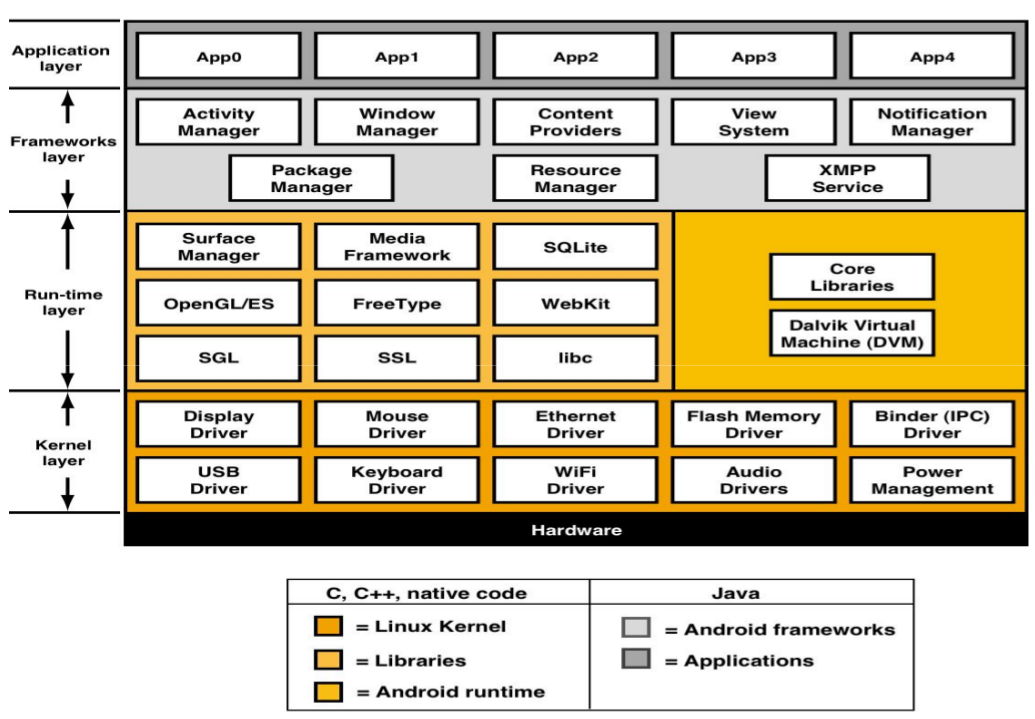
\includegraphics[scale=0.45]{project/images/system-architecture}
  \caption{\textbf{System Architecture}}
\end{figure}

Android Architecture is based on Linux 2.6 kernel. It helps to manage security,
memory management, process management, network stack and other important issues.
Therefore, the user should bring Linux in his mobile device as the main operating system and
install all the drivers required in order to run it. Android provides the support for the
Qualcomm MSM7K chipset family. For instance, the current kernel tree supports Qualcomm
MSM 7200A chipsets with stable version Qualcomm MSM 7200, which includes major
features:
\begin{itemize}
 \item WCDMA/HSUPA and EGPRS network support
 \item Bluetooth 1.2 and Wi-Fi support
 \item Digital audio support for mp3 and other formats
 \item Support for Linux and other third-party operating systems
 \item Java hardware acceleration and support for Java applications
 \item Qcamera up to 6.0 megapixels
 \item gpsOne – solution for GPS
 \item and lots of other features.
\end{itemize}

\section{Android and Synchronization}
\hspace*{0.82cm}The fast paced technology has changed the world as well as its habitants. In Today’s
global village there is no need to grab the telephone receiver and dial a specific number to
transmit voice through cables merely to hear the voice of a beloved. Now each of us carries
our own handsets with a built-in phonebook and text messages. The facilities like Wi-Fi and
internet have further improved the standard of communications by cutting down expenditure
and increasing availability.\\[0.5cm]
\hspace*{0.82cm}Regardless of the location, the world of web can be accessed through handsets,
laptops and tablet PCs. These modern times give us the necessity to maintain highly
important data on these portable devices so that we can access them on the go. But carrying
around this important data brings with it the risk of data getting corrupted due to hardware
failure, natural elements like rain spoiling our gadgets or the devices hard drive failing due to
shocks during transit.\\[0.5cm]
\hspace*{0.82cm}Hence to be safe and sure against such incidents it has become extremely to back up
our data after short intervals. Currently, the features of synchronization are available in
android devices, but they have a catch. These services are provided by third-party software
managers for e.g., Google.\\[0.5cm]
\hspace*{0.82cm}To back up our data, the data must be first synchronized with our Google account.
This means sending our extremely important data to the Google Clouds. This directly affects
the security and privacy aspects of the user. The data being stored on the Google cloud may
not be guarded securely. It is not guaranteed data will be safe and not private.\\[0.5cm]
\hspace*{0.82cm}Hence to overcome these restrictions, we have proposed a system where each user can
synchronize his/her phone with his/her own private server running anywhere. This will
ensure that all the data remains on our own private devices and no third-party can get hold of
this data.\\[0.5cm]
\hspace*{0.82cm}This means after synchronizing our private data like emails, SMS messages, contacts,
calendar entries, notes, documents, folders etc., all the data remains on the users server itself.
The server can be a Desktop Computer or a laptop connected to the internet. Also the android
devices can be synchronized in an offline manner.\\[0.5cm]
\hspace*{0.82cm}Offline sync can be done using Wi-Fi, Bluetooth or USB cable. Online sync will be
done via a secure connection over the internet. Using this product, the android user can be
ensured all their data remains on their own premises, no unnecessary sharing will be done to
third-parties, multiple copies of data can be maintained over multiple servers for additional
backup, if necessary.\\[0.3cm]

\begin{figure}[H]
  \centering
    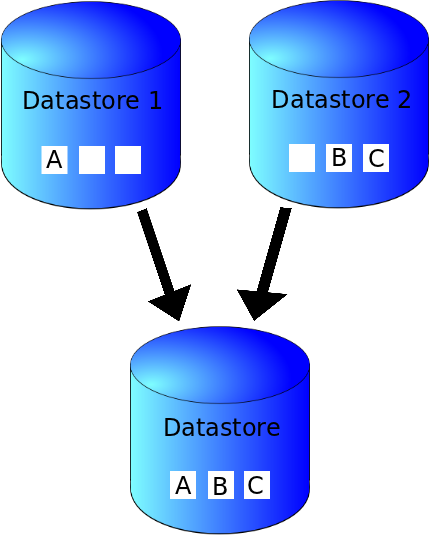
\includegraphics[height= 10cm, width=9cm]{project/images/data-sync}
  \caption{\textbf{Data Synchronization}}
\end{figure} % adds the Literature Survey page
\chapter{Software Requirements Specification}
\section{Introduction}
\subsection{Purpose}
\hspace*{0.82cm}This project aims at developing the Synchronization Manager for Android based devices.
Since there isn't any generic Synchronization Manger for android which works on all platforms
(Linux, Mac and Windows); this would help lots of people who work on two or more platforms. This
Synchronization Manager would be divided into two parts as server and client. The server would
reside on PC and client would be on Android Device. Client will gather information which is to be
synchronized.
\subsection{Document Conventions}
\hspace*{0.82cm}The following are the list of conventions and acronyms used in this document and the project as well,
privileges to the software:
\begin{itemize}
 \item \textbf{Client:} Intended users for the software.
 \item \textbf{SQL:} Structured Query Language; used to retrieve information from a database
 \item \textbf{SQL Server:} A server used to store data in an organized format
 \item \textbf{IEEE:} Institute of Electrical and Electronics Engineers
 \item \textbf{Layer:} Represents a section of the project
 \item \textbf{SYNC:} Synchronization
 \item \textbf{User Interface Layer:} The section of the assignment referring to what the user interacts with directly
 \item \textbf{Application Logic Layer:} The section of the assignment referring to the Web Server. This is where all 
computations are completed
 \item \textbf{Data Storage Layer:} The section of the assignment referring to where all data is recorded
 \item \textbf{Data flow diagram:} It shows the data flow between the entities
 \item \textbf{Use Case:} A broad level diagram of the project showing a basic overview
 \item \textbf{Boolean:} A true/false notation
 \item \textbf{Interface:} Something used to communicate across different mediums
\end{itemize}

\subsection{Intended Audience}
The intended audiences for this document are:
\begin{itemize}
 \item The team members of Innovative Android Synchronization Manager.
 \item The different Android users who are the clients.
\end{itemize}

This document will be reviewed frequently by the above audiences to check if the different
phases of the project are being completed by meeting the given requirements. If there are any changes
in the requirements in the course of the project they must be included in this document by making the
necessary changes.
\subsection{Product Scope}
\hspace*{0.82cm}The primary purpose of this is to have offline synchronization. At later stages this can be
extended to have online synchronization with services such as Ubuntu One for Linux. The software
can be made available as a paid service for corporations, users who want to backup their data.
\newpage
\section{Overall Description}
\subsection{Product Perspective}
\hspace*{0.82cm}Since at the moment there does not exist any generic android client for synchronizing data
off-line, this product will simplify synchronizing data across multiple mobile device manufacturers.
This is a new self-contained product. It is basically for android users who would like to have a generic
client for off-line and on-line synchronization of their data. This data may include information like
contacts, calendar entries, messages, notes, audio, video files. It is particularly useful for the careful
user who prefers synchronizing data on their own servers rather than a third-party service provider.
Also, it will benefit users of android who are concerned about sending data on third-party servers.\\[0.5cm]
The following diagram represents the proposed architecture:

\begin{figure}[H]
  \centering
    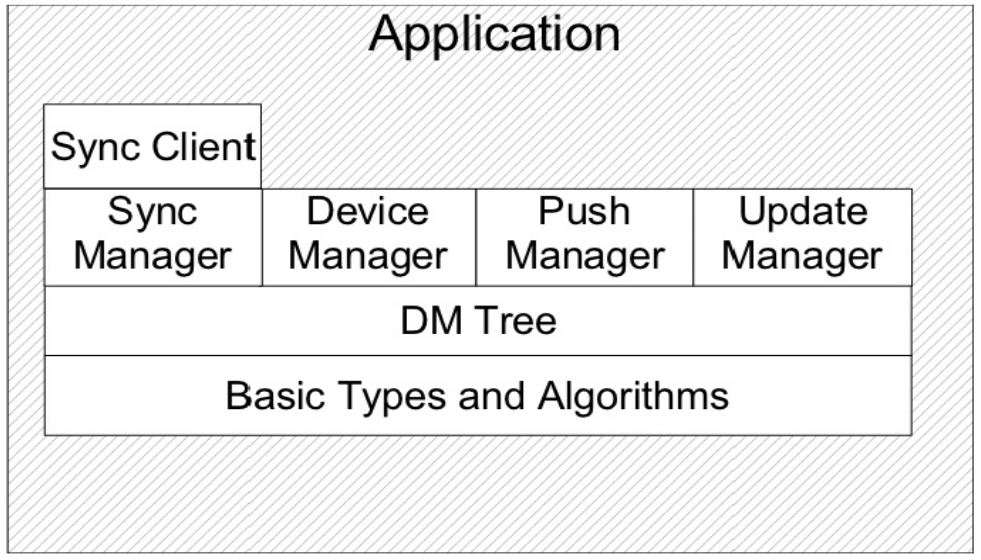
\includegraphics[scale=0.45]{project/images/client-architecture}
  \caption{\textbf{Architecture of Android Synchronization Manager (Client)}}
\end{figure}

\subsection{Product Functions}
\begin{itemize}
 \item Contact synchronization.
 \item Message synchronization.
 \item Calendar synchronization.
 \item Generating Reports.
 \item Managing logs of various activities in the phone (received/missed/dialed numbers).
 \item Backup of images, videos and other files.
\end{itemize}

\subsection{Operating Environment}
\begin{itemize}
 \item \textbf{For Client:} Android OS with v2.1 and above
 \item \textbf{For Server:} Qt 4.7+, SQLite
\end{itemize}

\subsection{Design and Implementation Constraints}
\hspace*{0.82cm}This is a product primarily being developed for users of a specific mobile platform i.e.
Android. Hence users of mobile phones apart from android cannot use the features of this product.
Also it may be a challenge to create synchronization of data between an android device and a device
running on some other platform. Hence these constraints cannot be overlooked. Fortunately, this
product will be designed in a way that it will be extensible for integrating synchronization feature for
other platforms of mobile devices.\\[0.5cm]
\hspace*{0.82cm}But taking into consideration the huge number of mobile phone manufacturers, adding this
feature may take a considerable amount of time. These additions can be added keeping in view the
popularity of the platform this product is being ported into. Also, online synchronization might be
slower for additional authentication features like use of SSL and other security features.

\subsection{User Documentation}
\hspace*{0.82cm}User documentation would include the built-in help which will give a step by step guidance to
users of the software on how to effectively use this product. Apart from this, an online help system
through e-mails or mailing lists can also be set up. The product will be developed with out-most
importance being given to simplicity so that minimum developer intervention would be needed for
maintenance.

\subsection{Assumptions and Dependencies}
\hspace*{0.82cm}While developing this product it is being assumed that the android platform version used would
be v2.1 [and above]. The usage of the same on a lower version may give unexpected results. But the
product will be developed to keep it as cross-platform compatible as possible.

\section{System Features}
\subsection{Synchronizing Contacts}
\hspace*{0.82cm}This feature is primarily why the product is being developed. This feature lets the user backup
contacts to the server. It will enable users to keep their server constantly updated with the newly
added contacts and their respective data.

\subsection{Synchronizing Messages}
\hspace*{0.82cm}This feature is basically used to backup SMSs and other drafts in the phone on to the server.
This feature is included as many users are keen on wanting to save all their conversations.

\subsection{Synchronizing files}
\hspace*{0.82cm}Along with all the data mentioned above, all the files on the user’s device can also be backed
up on the server. This will enable the user to store important information on the server and all the
information will be synchronized on a secure communication link.

\section{Analysis of Data}
\hspace*{0.82cm}All the information collected on Android operating system is obtained from
developer.android.com. Since Android is an open source, many of the codes are readily
available for application development, which has rapidly added to the success of Android
Systems. It gives budding engineers a platform for learning and development. The data
mentioned on the website developer.android.com explains the changes to be made in the
manifestation file for installing a new application. Moreover it explains the procedure of
connecting a USB device to Android supported phone. The two modes of android device viz.
Host mode and Accessory mode are mentioned on this website. These modes can be used for
offline synchronization of the data. The data obtained from this website proves to be
tremendously helpful in the android application development for the synchronization process.
\chapter{Requirement Analysis}
\section{User Side Requirements}
\begin{enumerate}
 \item User should have an android mobile device running OS version 2.1 or above.
 \item User should have Android Application installed within the mobile.
 \item User must be able to connect the device using USB cable
 \item User must be able to connect device using Wi-Fi.
 \item User must have internet plan enabled on his device or use Wi-Fi connection for
online synchronization.
 \item Interface must be user friendly and attractive.
\end{enumerate}

\section{System Side Requirements}
\begin{enumerate}
 \item System must have Android based drivers for USB and Wi-Fi adapters.
 \item The server side application must be installed on the standard PC.
 \item System must be connected to the internet for online synchronization.
 \item Interface must be user friendly and attractive.
\end{enumerate}

\section{Hardware and Software Requirements}
\begin{enumerate}
 \item Android Based Mobile with minimum of:
 \begin{enumerate}[a. ]
  \item 128KB non-volatile memory to run Mobile Information Device (MID).
  \item 8KB of non-volatile memory for storage of persistent application data.
  \item 2KB of volatile memory to run JVM
 \end{enumerate}
 \item Device should have Wi-Fi connectivity.
 \item 600mhz processor
 \item 150 MB of RAM
\end{enumerate}

\section{Non-functional Requirement}
\subsection{Security Requirements}
\hspace*{0.82cm}In our product, security is of out-most importance. Hence we need to implement
communication over HTTPS. For that it is required that the user should be in an environment where
the HTTPS port is not blocked. In case these ports are not enabled, an http connection will have to be
used. This means using http instead of https would lead to vulnerability of the user’s data to be sniffed
by third-party. Hence this should be considered as a security requirement of the product.
\subsection{Performance Requirements}
The main requirement here is a good communication. If the communication lags, the purpose of the software 
is defeated. However, this requirement is mostly a issue at the client end.
\subsection{Safety Requirements}
This product requires some safety concerns. The handshaking between client and server in bluetooth mode should 
be secure.
\newpage
\section{External Interface Requirements}
\subsection{Hardware Interfaces}
\hspace*{0.82cm}Typical hardware interfaces that would be required would be the standard USB data cable
provided with the device. No other additional hardware interfacing would be needed to be bought by
the user. Also Bluetooth and/or Wi-Fi adapter on the server machine would be needed for
communication (in case USB cable is not available). Communication protocol would be developer
implemented and the user need not worry about communicating using this protocol. Hence this
product will be extremely user-friendly.

\subsection{Software Interfaces}
\hspace*{0.82cm}The product featured, requires a database to be maintained at both the ends - client and server.
Hence we will be deploying two different databases on both of them which will be in sync on
demand.\\[0.5cm]
\hspace*{0.82cm}The client DB will be implemented using SQLite and the server DB will be standard
PostgreSQL. The UI on client will be a typical android user interface using the default options
available at the time of development. UI on server will be implemented using Qt and python at the
backend.

\subsection{Communications Interfaces}
\hspace*{0.82cm}This product basically works on the client-server architecture. Hence a communication
mechanism between server and client has to be developed. This communication will be established
over https or local Bluetooth or Wi-Fi. USB cable is another option. E-mails can be used to
send/receive reports, log files.
\chapter{System Design}
\section{Goals of Design}
\begin{enumerate}
 \item The project design should help us to visualize the system as it is or want it to be.
 \item It should permit us to specify the structure or behavior of the system.
 \item To give us template that guides us in the construction of the system.
 \item To document the decision we have made.
\end{enumerate}

\section{UML Diagrams}
\hspace*{0.82cm}The OMG's Unified Modeling Language (UML) helps specify, visualize, and
document models of software systems, including their structure and design, in a way that
meets all of these requirements. Using any one of the large number of UML-based tools on
the market, one can analyze future application's requirements and design a solution that meets
them, representing the results using UML's twelve standard diagram types. One can model
just about any type of application, running on any type and combination of hardware,
operating system, programming language, and network, in UML. Its flexibility helps model
distributed applications that use just about any middleware on the market. Built upon the
MOF metamodel which defines class and operation as fundamental concepts, it's a natural fit
for object-oriented languages and environments such as C++, Java and the recent C\#, but one
can use it to model non-OO applications as well in, for example, Fortran, VB, or COBOL.\\[0.5cm]
\hspace*{0.82cm}Architects design buildings. Builders use the designs to create buildings. The more
complicated the building, the more critical the communication between architect and builder.
Blueprints are the standard graphical language that both architects and builders must learn as
part of their trade.\\[0.5cm]
\hspace*{0.82cm}Writing software is not unlike constructing a building. The more complicated the
underlying system, the more critical the communication among everyone involved in creating
and deploying the software. In the past decade, the UML has emerged as the software
blueprint language for analysts, designers, and programmers alike. It is now part of the
software trade. The UML gives everyone from business analyst to designer to programmer a
common vocabulary to talk about software design.\\[0.5cm]
\hspace*{0.82cm}The UML is applicable to object-oriented problem solving. Anyone interested in
learning UML must be familiar with the underlying tenet of object-oriented problem solving 
it all begins with the construction of a model. A model is an abstraction of the underlying
problem. The domain is the actual world from which the problem comes.\\[0.5cm]
\hspace*{0.82cm}Models consist of objects that interact by sending each other message. Think of an
object as "alive." Objects have things they know (attributes) and things they can do
(behaviors or operations). The values of an object's attributes determine its state.\\[0.5cm]
\hspace*{0.82cm}Classes are the "blueprints" for objects. A class wraps attributes (data) and behaviors
(methods or functions) into a single distinct entity. Objects are instances of classes.\\[0.5cm]
At the center of the UML are its nine kinds of modeling diagrams, which we describe here.
\begin{itemize}
 \item Use case diagrams
 \item Class diagrams
 \item Object diagrams
 \item Sequence diagrams
 \item Collaboration diagrams
 \item Statechart diagrams
 \item Activity diagrams
 \item Component diagrams
 \item Deployment diagrams
\end{itemize}
To model our system we have used the following diagrams:\\[0.5cm]
\textbf{Class Diagram}\\
\hspace*{0.82cm}A Class diagram is type of structure diagram that describes
structure of our system by showing system classes, their attributes and relationships between
them. Class diagrams are important for visualizing, specifying and documenting structural
models.\\[1cm]
\begin{figure}[H]
  \centering
    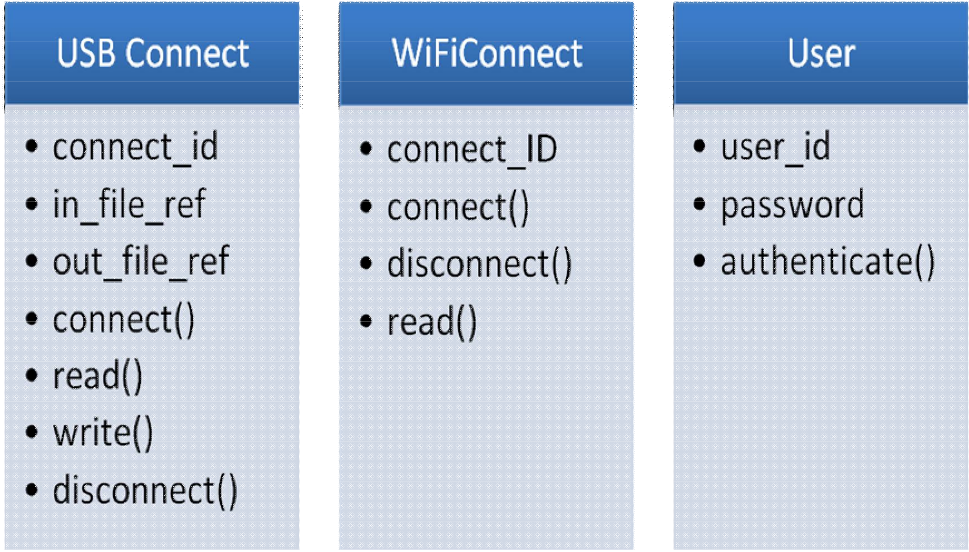
\includegraphics[height= 8cm, width=15cm]{project/images/class-diagram}
  \caption{\textbf{Class Diagram}}
\end{figure}
\newpage
\textbf{Use Case Diagram}\\
\hspace*{0.82cm}Use case diagram are central to modeling the behavior of a system or class each one
shows a set of use cases and actors and their relationships. These model the users expectation
for using the system.\\[1cm]
\begin{figure}[H]
  \centering
    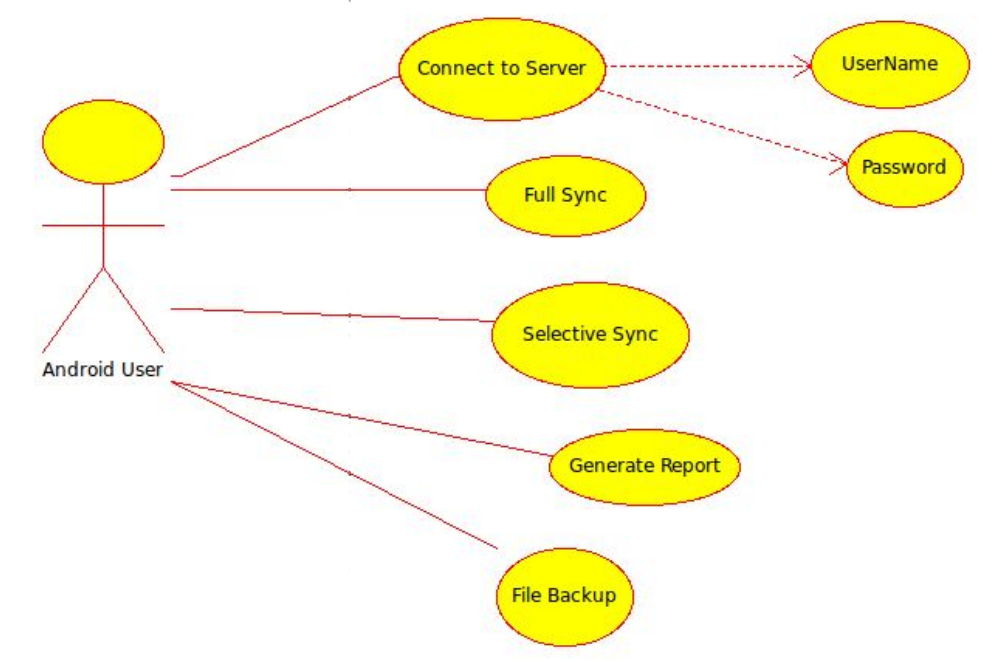
\includegraphics[height= 15cm, width=15cm]{project/images/use-case}
  \caption{\textbf{Use Case Diagram}}
\end{figure}
\newpage
\textbf{Sequence Diagram}\\
\hspace*{0.82cm}A sequence diagram in a Unified Modeling Language (UML) is a kind of interaction
diagram that shows how processes operate with one another and in what order. It is a
construct of a Message Sequence Chart. A sequence diagram shows object interactions
arranged in time sequence. It depicts the objects and classes involved in the scenario and the
sequence of messages exchanged between the objects needed to carry out the functionality of
the scenario. Sequence diagrams typically are associated with use case realizations in the
Logical View of the system under development.\\[1cm]
\begin{figure}[H]
  \centering
    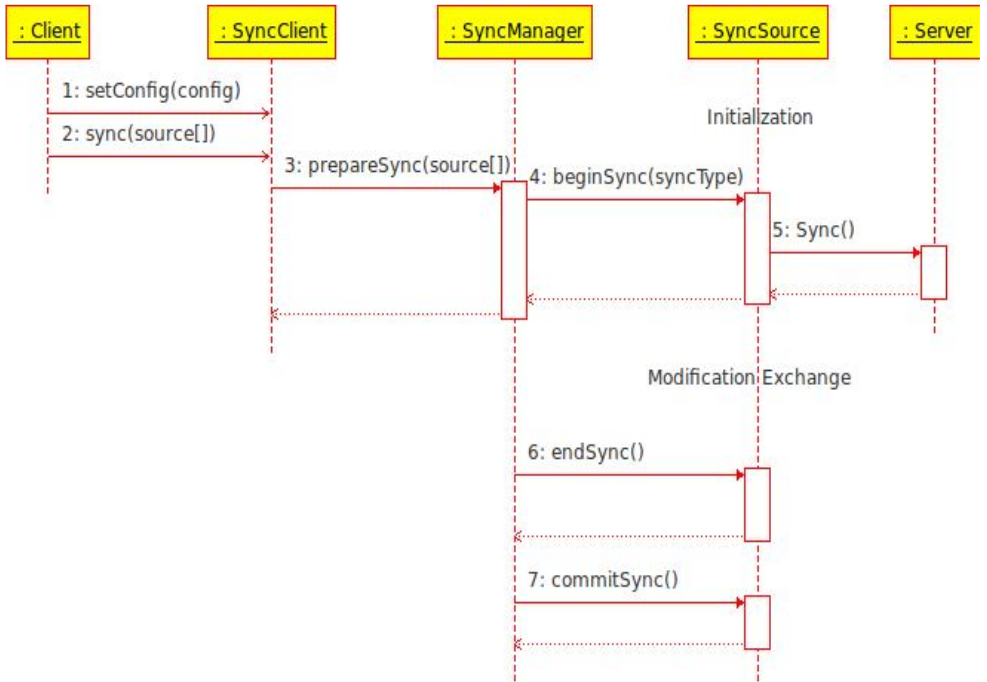
\includegraphics[height= 15cm, width=17cm]{project/images/seq-diagram}
  \caption{\textbf{Sequence Diagram}}
\end{figure}
%\chapter{Proposed Work}

\section{Problem Statement}
XXXXXXX

\section{Module1}
XXXXXXX
\subsection{SubSection1}
XXXXXXX % adds the Project Work page
%\chapter{Research Methodology}

\section{Module1}

\subsection{Subsection}
XXXXXXX
\subsubsection{SubSub}
XXXXXXXXXXXXXXXXXXXXX     % adds the Research Methodology page
\chapter{Implementation}

\section{Module1}

\subsection{Submodule1}
Code Snippet
\lstinputlisting{project/helloworld.py}
XXXXXXXXXXXXXXXXXXXXX % adds the Project Design
%\chapter{Scheduling}


\section{Proposed Modules}

XXXXXXX
\section{Scheduling}

XXXXXXX % adds the Scheduling and Planning page
\chapter{Conclusion and Future Scope}
\section{Conclusion}
\hspace*{0.82cm}Android operating system is still in its infancy despite of some tremendous progress.
The proposed system focuses on some important and fruitful technologies which may assist
human race in easier interaction with the digital world. This system has ample scope in the
android market where millions of users download and use software on a daily basis.
Furthermore the future work could draw in research on similar operations using Java-
powered devices.
\section{Future Scope}
\begin{itemize}
 \item Support Java Platforms: Create application for Java supported phones due to be wide
availability.
 \item Making system compact to increase flexibility, portability
 \item Extend application to support J2ME devices.
 \item Make similar server application that can be run another android phone instead of PC.
 \item Animation of user interactions for simplified use.
 \item Integrate other features like controlling android device from PC.
\end{itemize}
 % adds the Scheduling and Planning page
\addcontentsline{toc}{chapter}{References}
\begin{thebibliography}{99}
\bibitem{MoSync} \emph{MoSync: A synchronization scheme for cellular wireless and mobile multimedia systems}; Azzendine Boukerche, 
Sungbum Hong and Tom Jacob
\bibitem{SyncML} \emph{Data Synchronization Protocol in Mobile Computing Environment Using SyncML}; Byung-Yun Lee, Tae-Wan Kim, Dae-Woong Kim and 
Hoon Choi
\bibitem{AndroidDeveloper} \url{http://developer.android.com}
\bibitem{Funambol} \url{http://funambol.org}
\bibitem{OpenSync} \url{http://opensync.org}
\bibitem{Wikipedia} \url{http://en.wikipedia.org/wiki/SyncML}
\bibitem{Qt} \url{http://doc.qt.nokia.com/latest/tutorials.html}
\end{thebibliography} % adds the References page

%}\end{spacing}
\end{document}
